\subsection{ELEMENT}

\paragraph{Fighting Wing}
\textbf{Easiest for wingman} --- used in low-threat areas

\begin{multicols}{2}
\textbf{Advantages}
\begin{itemize}
    \item easy to maintain
    \item leader's 6'o'clock covered
    \item allows heads-down time
\end{itemize}
\columnbreak
\textbf{Disadvantages}
\begin{itemize}
    \item wingman's 6'o'clock NOT covered
    \item close proximity
\end{itemize}
\end{multicols}

\hfill\textbf{Reference \cref{fig:supp_fig:form:fightingwing}}

\paragraph{Wedge}
\textbf{Similar to fighting wing} --- more spaced out

\begin{multicols}{2}
    \textbf{Advantages}
    \begin{itemize}
        \item easy to maintain
        \item leader's 6'o'clock covered
        \item free for aggressive maneuvering
    \end{itemize}
    \columnbreak
    \textbf{Disadvantages}
    \begin{itemize}
        \item wingman's 6'o'clock NOT covered
        \item lead changes difficult
    \end{itemize}
\end{multicols}

\hfill\textbf{Reference \cref{fig:supp_fig:form:wedge}}

\begin{figure}[htbp]
    \centering
    \begin{minipage}[b]{0.5\textwidth}
        \centering
        \begin{tikzpicture}[figstyle]
            
            \coordinate (lead) at (0,0);
            \coordinate (wing) at ($(lead)+(-45:27.5)$);
    
            \draw[dashed]
            (lead) -- ++(-30:15) arc (-30:-60:15) -- (lead);
    
            \draw[fill=color2!15]
            ($(lead)+(-30:15)$) 
            -- ++(-30:25) node[font=\footnotesize, pos=1, right] {30$^\circ$}
            arc  (-30:-60:40) 
            node[font=\footnotesize, below, pos=0.5, rotate=45] {0.5nm}
            node[font=\footnotesize, pos=1, below right] {60$^\circ$}
            -- ++(120:25)
            arc (-60:-30:15)
            node[font=\footnotesize, below, pos=0.5, rotate=45] {0.1nm};
    
            \node[yshift=-3mm] (leadfig) at (lead) {
                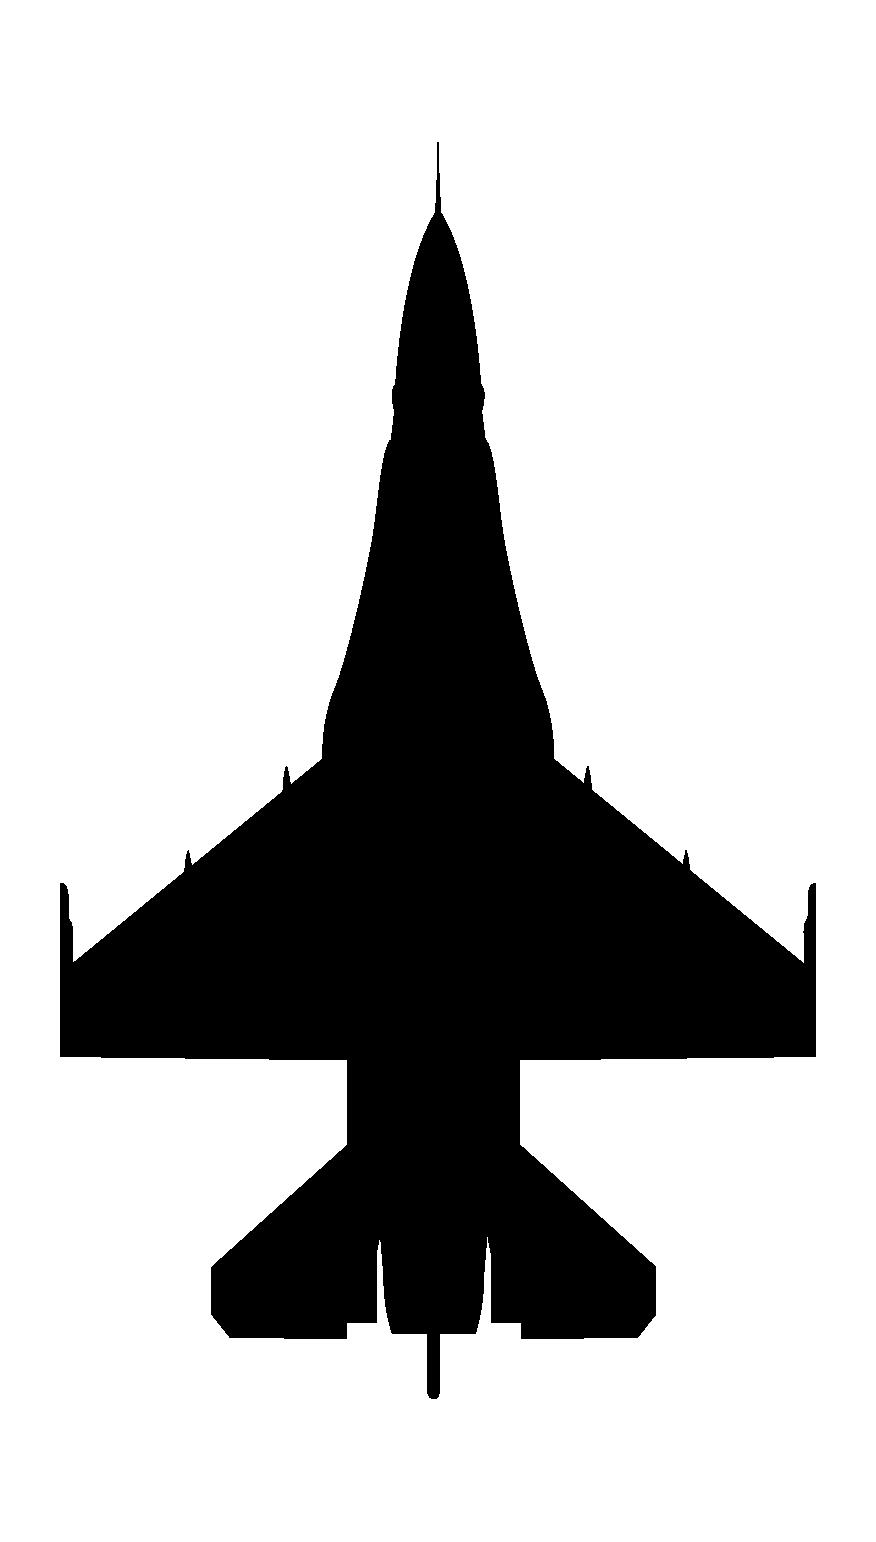
\includegraphics[
                    width=7.5mm,
                ]{diagrams/aircraft/silhouette_f16_top.pdf}
            };
            
            \node[] (wingfig) at (wing) {
                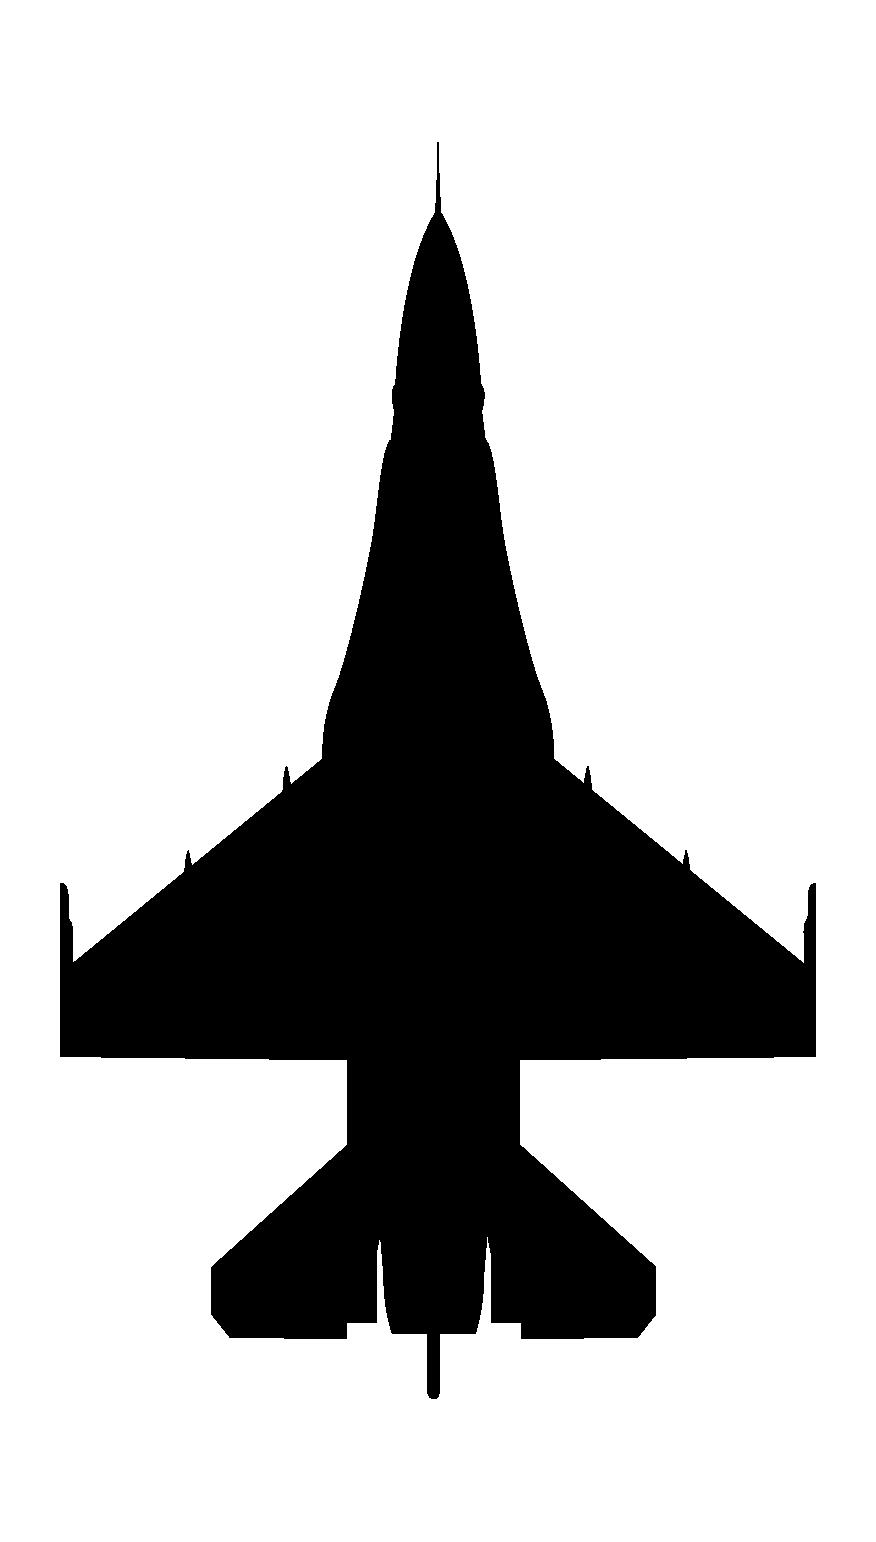
\includegraphics[
                    width=7.5mm,
                ]{diagrams/aircraft/silhouette_f16_top.pdf}
            };
    
        \end{tikzpicture}
        \caption{Fighting wing}
        \label{fig:supp_fig:form:fightingwing}
    \end{minipage}%
    \begin{minipage}[b]{0.5\textwidth}
        \centering
        \begin{tikzpicture}[figstyle]
            
            \coordinate (lead) at (0,0);
            \coordinate (wing) at ($(lead)+(-45:30)$);
    
            \draw[dashed]
            (lead) -- ++(-30:20) arc (-30:-60:20) -- (lead);
    
            \draw[fill=color2!15]
            ($(lead)+(-30:20)$) 
            -- ++(-30:20) node[font=\footnotesize, pos=1, right] {30$^\circ$}
            arc  (-30:-60:40) 
            node[font=\footnotesize, below, pos=0.5, rotate=45] {1.0 nm}
            node[font=\footnotesize, pos=1, below right] {60$^\circ$}
            -- ++(120:20)
            arc (-60:-30:20)
            node[font=\footnotesize, below, pos=0.5, rotate=45] {0.5 nm};
    
            \node[yshift=-3mm] (leadfig) at (lead) {
                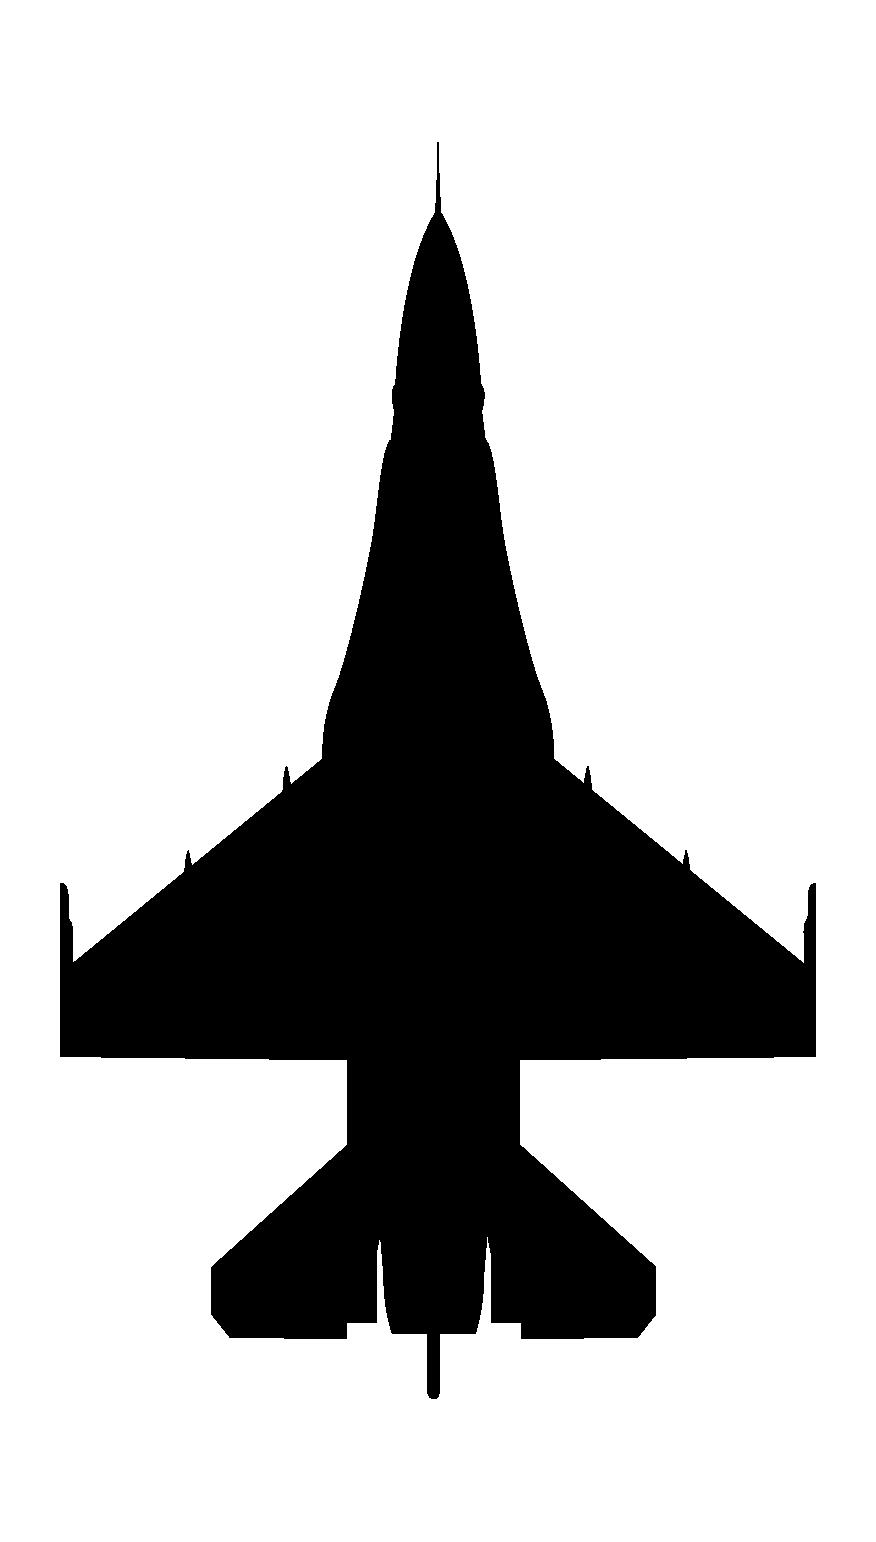
\includegraphics[
                    width=7.5mm,
                ]{diagrams/aircraft/silhouette_f16_top.pdf}
            };
            
            \node[] (wingfig) at (wing) {
                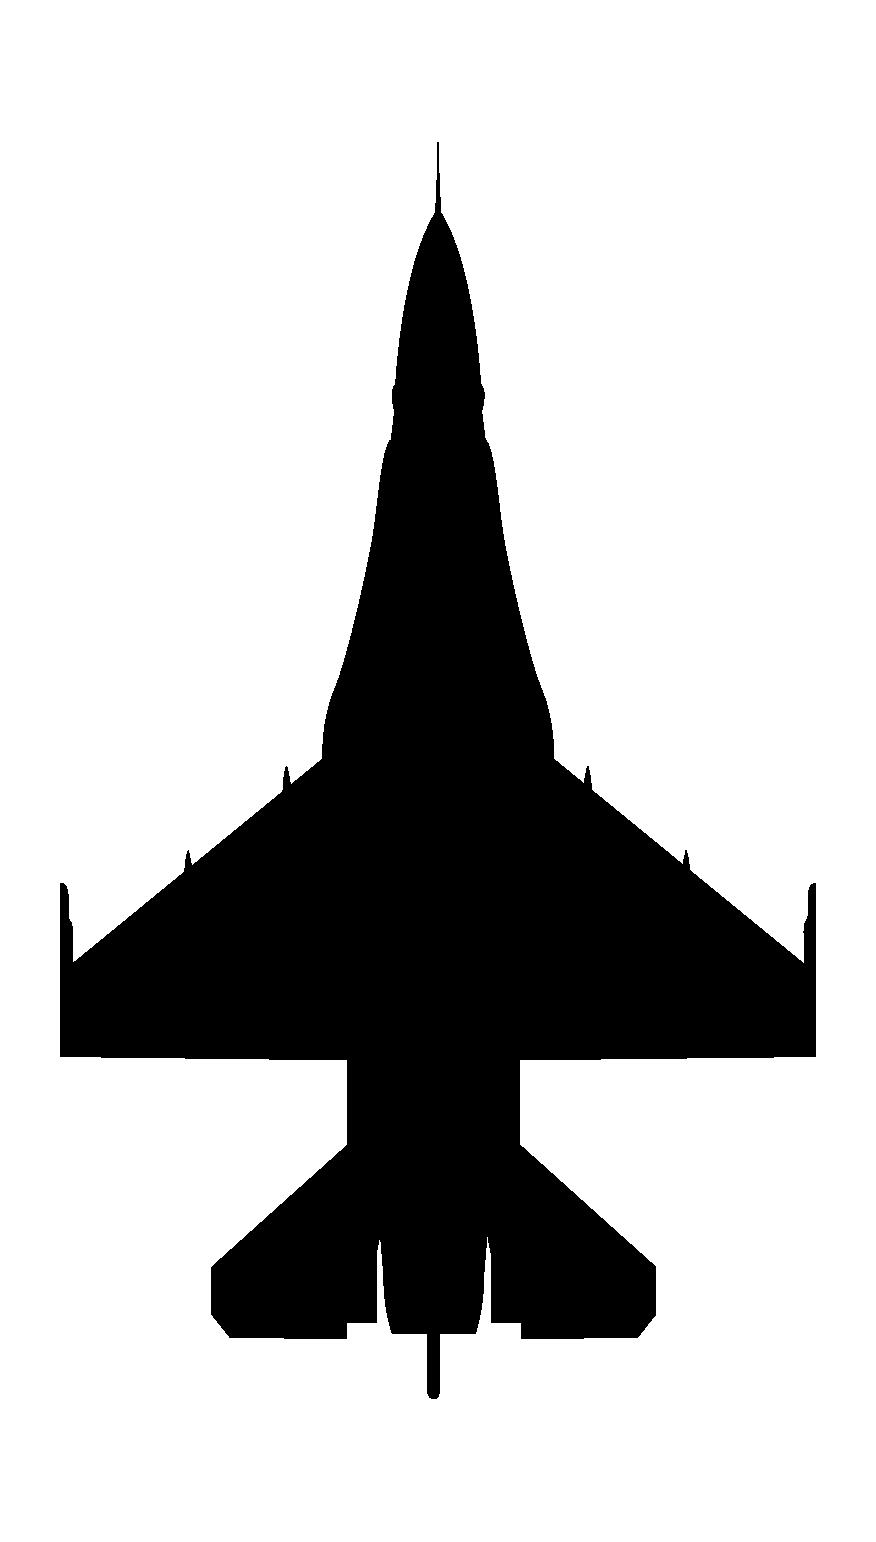
\includegraphics[
                    width=7.5mm,
                ]{diagrams/aircraft/silhouette_f16_top.pdf}
            };
    
        \end{tikzpicture}
        \caption{Two-ship wedge}
        \label{fig:supp_fig:form:wedge}
    \end{minipage}

    \vspace{2em}
    \begin{minipage}[b]{0.55\textwidth}
        \centering
        \begin{tikzpicture}[figstyle]
        
            \coordinate (lead) at (0,0);
            \coordinate (wing) at ($(lead)+(0:40)$);
    
            \draw[dashed]
            (lead) -- ++(0:20) arc (0:-20:20) -- (lead);
    
            \draw[fill=color2!15]
            ($(lead)+(0:20)$) 
            -- ++(0:40) node[font=\footnotesize, pos=1, right] {0$^\circ$}
            arc  (0:-20:60) 
            node[font=\footnotesize, right, pos=0.5] {2.0 nm}
            node[font=\footnotesize, pos=1, below right] {20$^\circ$}
            -- ++(160:40)
            arc (-20:0:20)
            node[font=\footnotesize, right, pos=0.5] {0.7 nm};
    
            \node[yshift=-3mm] (leadfig) at (lead) {
                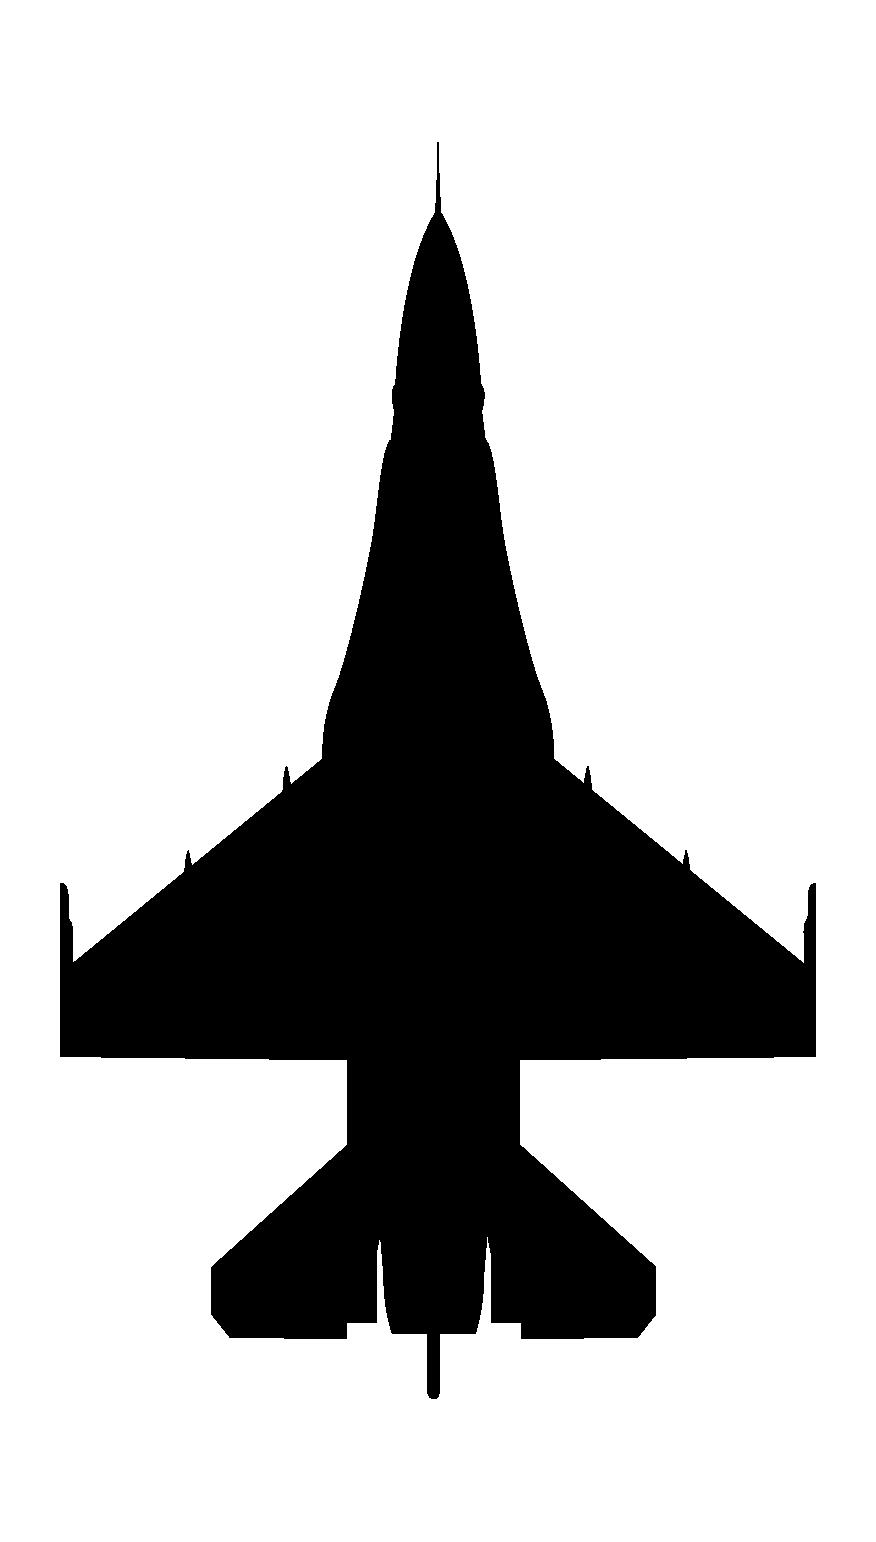
\includegraphics[
                    width=7.5mm,
                ]{diagrams/aircraft/silhouette_f16_top.pdf}
            };
            
            \node[yshift=-3mm] (wingfig) at (wing) {
                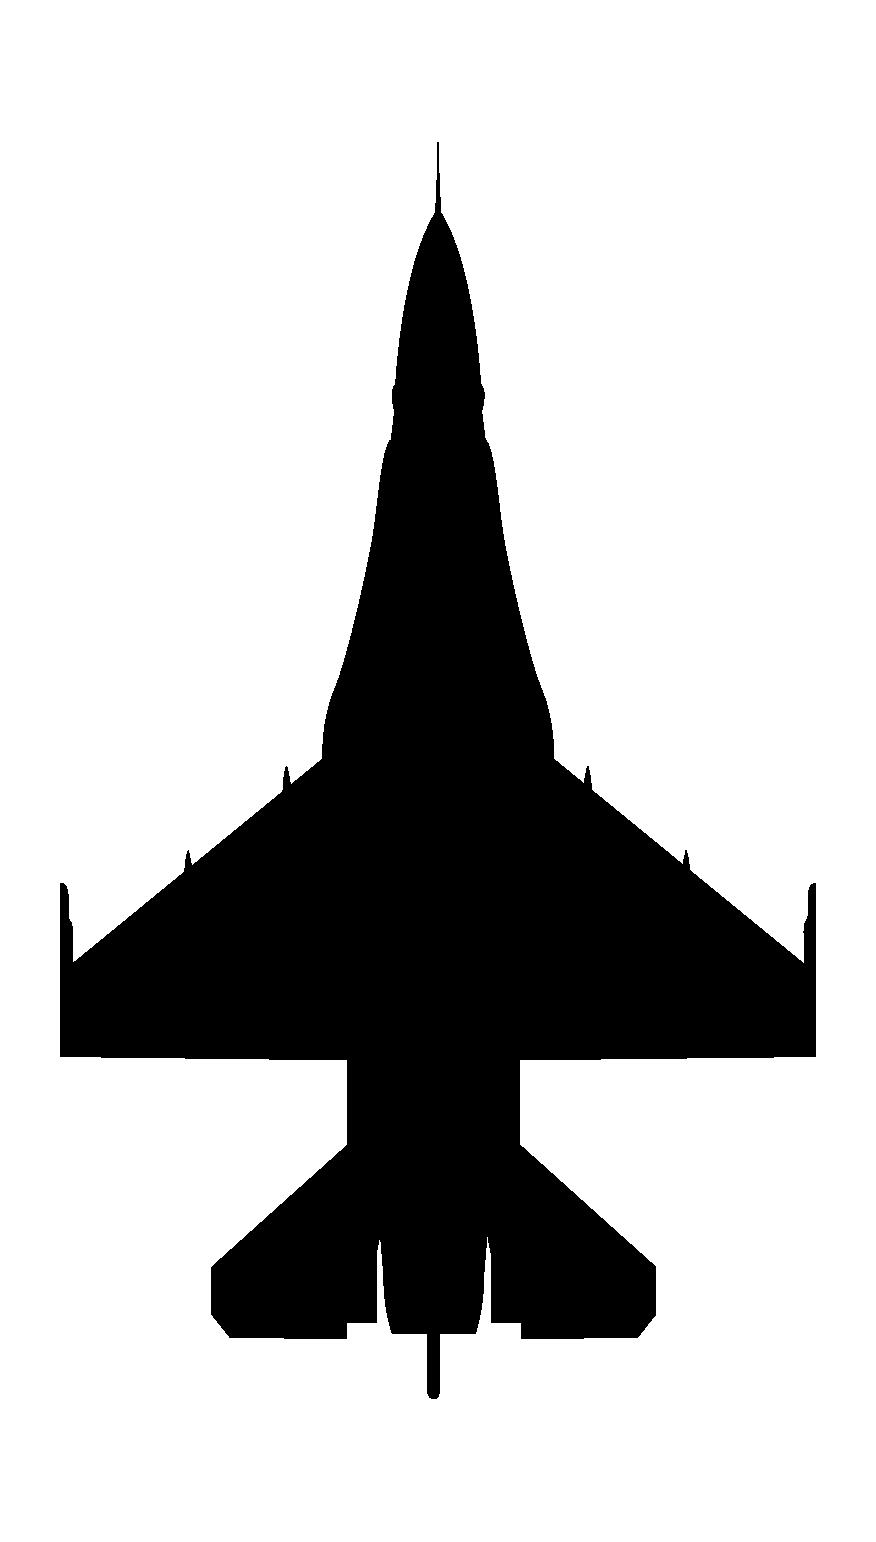
\includegraphics[
                    width=7.5mm,
                ]{diagrams/aircraft/silhouette_f16_top.pdf}
            };
    
        \end{tikzpicture}
        \caption{Two-ship line abreast (LAB)}
        \label{fig:supp_fig:form:lineabreast}
    \end{minipage}%
    \begin{minipage}[b]{0.45\textwidth}
        \centering
        \begin{tikzpicture}[figstyle]
        
            \coordinate (lead) at (0,0);
            \coordinate (wing) at ($(lead)+(-30:30)$);
    
            \draw[dashed]
            (lead) -- ++(0:20) arc (0:-60:20) -- (lead);
    
            \draw[fill=color2!15]
            ($(lead)+(0:20)$) 
            -- ++(0:20) node[font=\footnotesize, pos=1, right] {0$^\circ$}
            arc  (0:-60:40) 
            node[font=\footnotesize, right, pos=0.5] {2.0 nm}
            node[font=\footnotesize, pos=1, below right] {60$^\circ$}
            -- ++(120:20)
            arc (-60:0:20)
            node[font=\footnotesize, right, pos=0.75] {1.0 nm};
    
            \node[yshift=-3mm] (leadfig) at (lead) {
                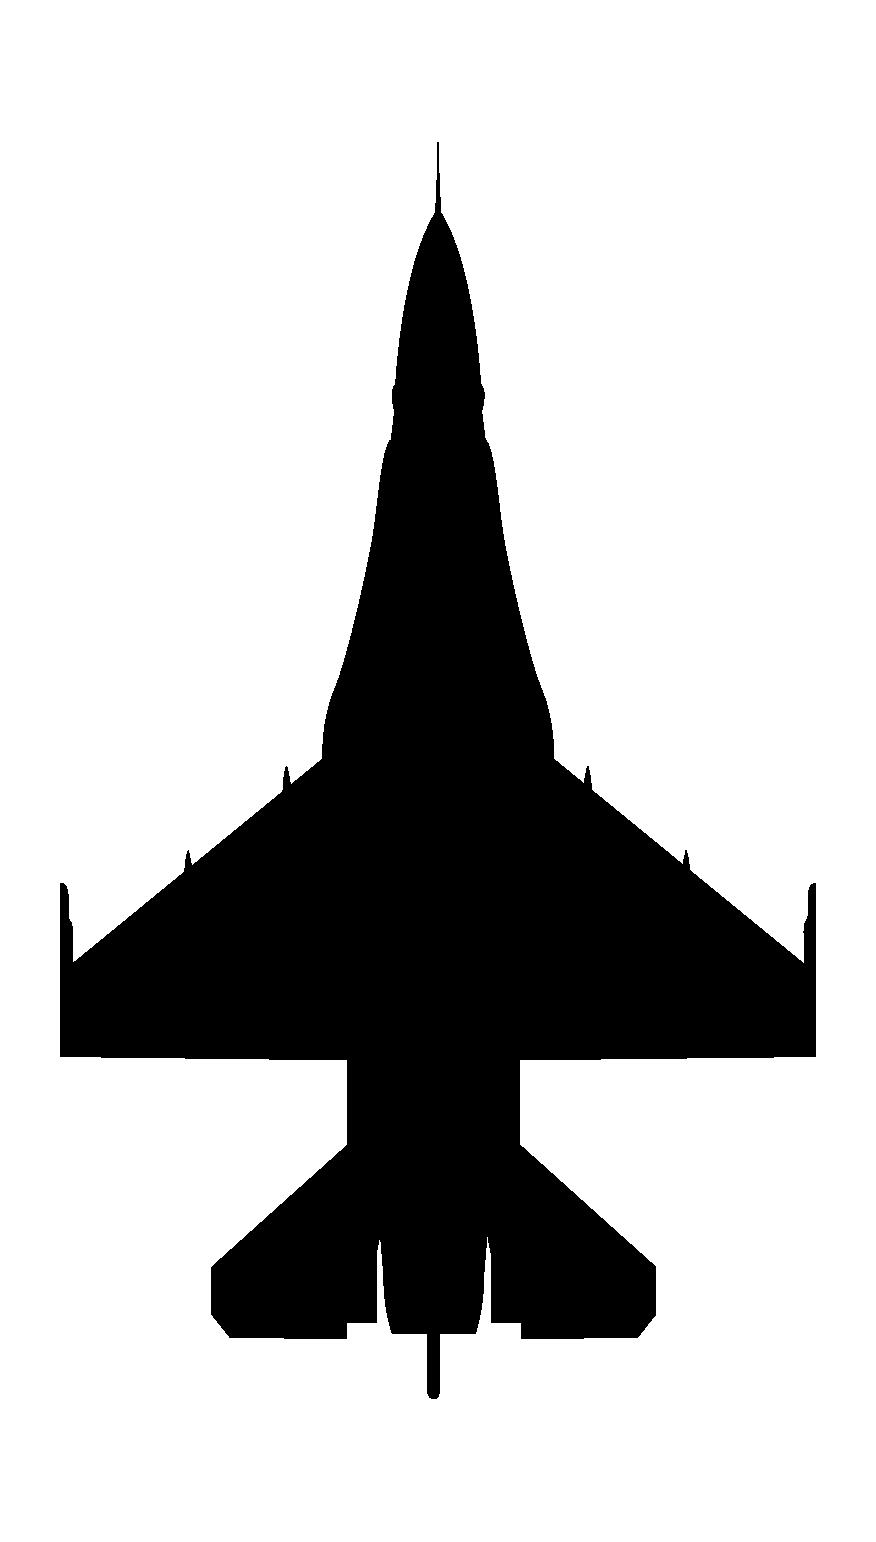
\includegraphics[
                    width=7.5mm,
                ]{diagrams/aircraft/silhouette_f16_top.pdf}
            };
            
            \node[yshift=-0mm] (wingfig) at (wing) {
                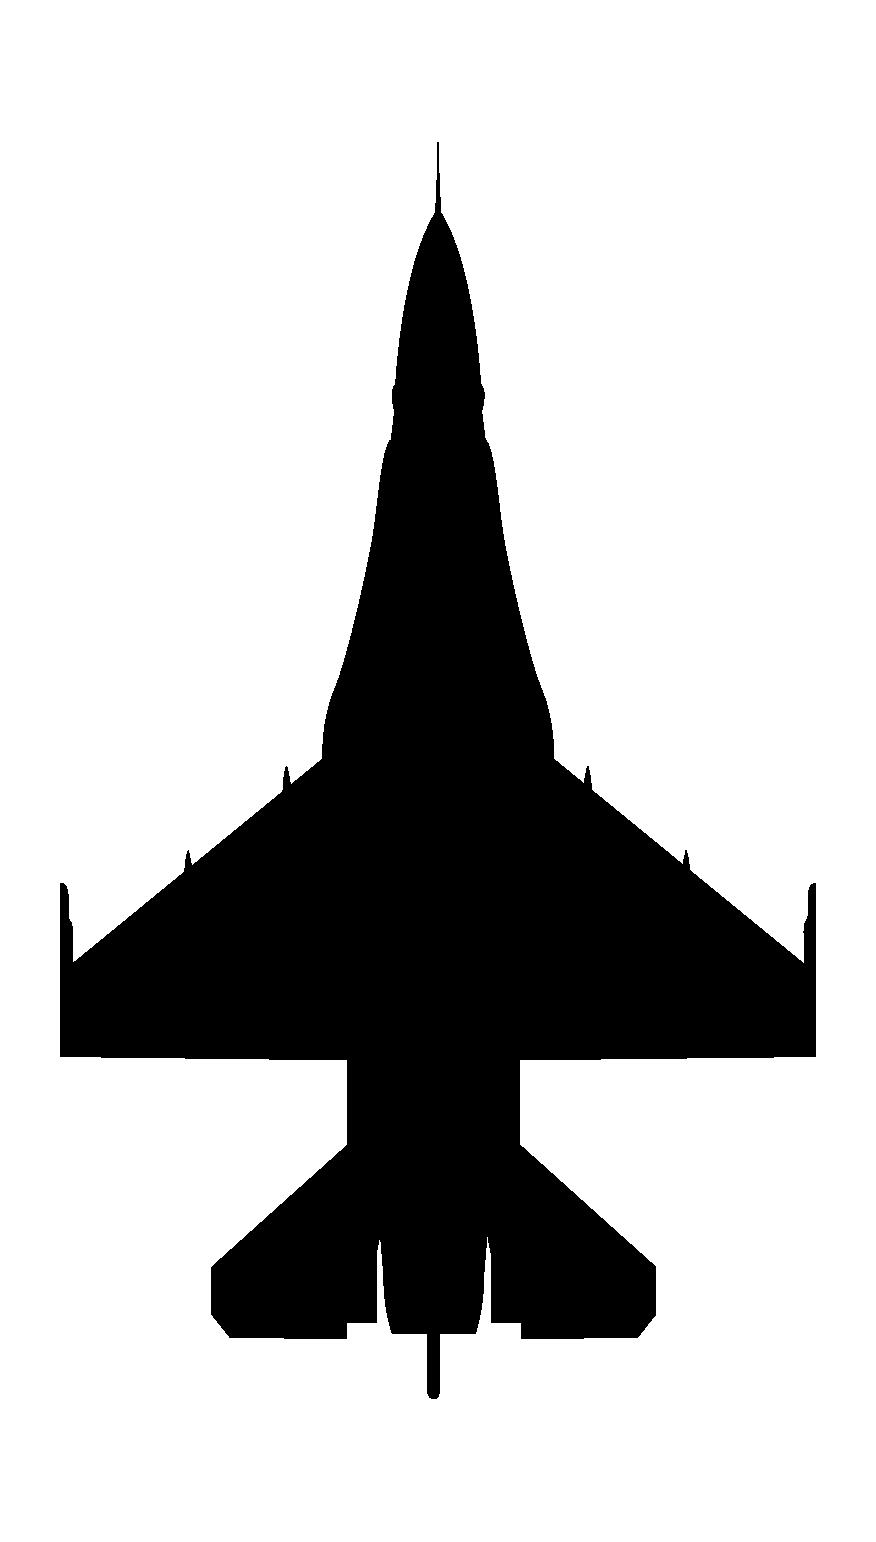
\includegraphics[
                    width=7.5mm,
                ]{diagrams/aircraft/silhouette_f16_top.pdf}
            };
    
        \end{tikzpicture}
        \caption{Two-ship spread}
        \label{fig:supp_fig:form:spread}
    \end{minipage}
\end{figure}

\paragraph{Line Abreast \break LAB}
\textbf{Tactical A-A formation} --- mutual 6'o'clock cover, ensures all flight members in position to shoot simultaneously

\begin{multicols}{2}
\textbf{Advantages}
\begin{itemize}
    \item mutual 6'o'clock cover
    \item laterally spread
    \item simplifies tactical turns
    \item allows simultaneous bandit engagement
\end{itemize}
\columnbreak
\textbf{Disadvantages}
\begin{itemize}
    \item requires continuous monitoring to maintain
\end{itemize}
\end{multicols}

\hfill\textbf{Reference \cref{fig:supp_fig:form:lineabreast}}

\paragraph{Spread}
\textbf{Similar to line abreast} --- more room for wingman to maneuver

\hfill\textbf{Reference \cref{fig:supp_fig:form:spread}}

\clearpage